\documentclass[12pt,fleqn]{article}
\usepackage{vkCourseML}
\usepackage{gensymb}
\hypersetup{unicode=true}
%\usepackage[a4paper]{geometry}
\usepackage[hyphenbreaks]{breakurl}

\interfootnotelinepenalty=10000

\begin{document}
\title{Лекция 19\\Частичное обучение}
\author{Е.\,А.\,Соколов\\ФКН ВШЭ\\\normalsize{tex by Н. Морозов}}
\maketitle

Представим, что у нас есть обучающая выборка $X^\ell = \{(x_i, y_i)\}_{i = 1}^{\ell}$, но помимо нее также имеется неразмеченная выборка $X^u = \{x_i\}_{i = \ell + 1}^{n}$. И для обучения модели нам хотелось бы использовать данные обоих видов. Ситуация вполне естественная, так как зачастую бывает, что собрать неразмеченные данные гораздо проще, чем их разметить.

Пояснить идею частичного обучения можно на следующем примере. Пусть среди размеченных данных у нас есть два небольших облака точек: зеленое и красное. Они находятся достаточно далеко друг от друга, так что мы с легкостью могли бы провести разделяющую гиперплоскость посередине. При этом у нас есть заметно большее количество неразмеченных данных, назовем их серыми точками. После добавления серых точек, каждое облако заметно расширяется, но они все еще отделены друг от друга. И хоть мы формально не знаем, какого цвета должна быть каждая из серых точек, новые формы облаков нам говорят, что разделяющую гиперплоскость на самом деле неплохо бы провести в другом месте.

\begin{center}
    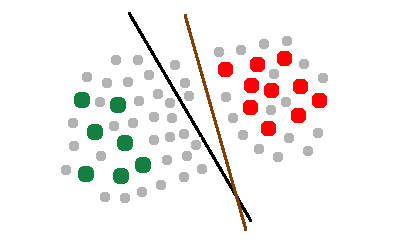
\includegraphics[width=0.47\textwidth]{semi-supervised_example.png}
\end{center}

\section{Self-training}

Рассмотрим следующий алгоритм:
\begin{enumerate}
    \item Обучить модель $a(x)$ на $X^\ell$
    \item Применить $a(x)$ на $X^u$
    \item Добавить $(x_i, a(x_i))$ к $X^\ell$ для некоторых $x_i \in X^u$
    \item Вернуться к шагу $1.$
\end{enumerate}
В пункте 3, в случае классификации, можно например добавлять объекты, на которых модель имеет наибольшую уверенность. Также можно добавлять объекты, близкие к $X^\ell$. При этом просто добавить все объекты из $X^u$ может быть плохой идеей, так как если в неразмеченной выборке есть выбросы, мы только подпортим себе жизнь. Помочь бороться с этой проблемой может добавление в целевой функционал весов, равных уверенностям модели в предсказаниях на $X^u$.

\section{Генеративные подходы}

Предположим, что на наших данных есть распределение $p(x, y \cond \theta) = p(y \cond \theta)p(x \cond y, \theta)$. Например, в случае нормального распределения в $\theta$ будут средние и ковариационные матрицы для всех классов. И если бы у нас была только выборка $X^\ell$, мы бы просто максимизировали правдоподобие
\[
    \sum\limits_{i = 1}^{\ell} \log \left(p(y_i \cond \theta)p(x_i \cond y_i, \theta)\right) \to \max_\theta.
\]

Давайте теперь скажем, что неразмеченные данные мы будем описывать в виде смеси распределений всех классов. Тогда задачу максимизации правдоподобия можно записать как
\[
    \sum\limits_{i = 1}^{\ell} \log \left(p(y_i \cond \theta)p(x_i \cond y_i, \theta)\right) + \sum\limits_{i = \ell + 1}^{n} \log \left(\sum\limits_{y = 1}^k p(y \cond \theta) p(x_i \cond y, \theta)\right) \to \max_\theta.
\]
Для оптимизации по $\theta$ используем EM-алгоритм.

Заметим, что неразмеченных данных у нас обычно куда больше, чем размеченных, поэтому второе слагаемое в формуле будет сильно перевешивать первое. Тогда мы по итогу просто будет решать задачу подгонки распределения под неразмеченную выборку. Для решения этой проблемы можно вставить костыль в виде домножения второго слагаемого в функционале на некоторый гиперпараметр $\lambda < 1$.

\subsection{cluster-and-label}

В упрощенной версии мы можем обучить какой-нибудь алгоритм кластеризации на $X^\ell \cup X^u$ и в каждом кластере неразмеченным объектам выдать класс, наиболее популярный в этом кластере. 

\section{Методы на основе моделей}

\subsection{Логистическая регрессия}

Существует некоторое обобщение логистической регрессии, называемое обобщенными линейными моделями, и есть способ встроить туда неразмеченные данные, называемый Expectation Regularization. Но этот подход мы тут рассматривать не будем.

\subsection{SVM}

Подход на основе SVM называется Semi-supervised SVM, или S3VM. Вспомним вариант безусловной задачи оптимизации обычного SVM с hinge loss
\[
\|w\|^2 + C \sum\limits_{i = 1}^\ell \max(0, 1 - y_i \langle w, x_i \rangle) \to \min_{w}
\]

Попробуем теперь каким-то образом штраф за неразмеченные объекты. Давайте скажем, что они не должны находиться слишком близко к разделяющей гиперплоскости. Тогда получится следующая задача оптимизации:
\[
\|w\|^2 + C_1 \sum\limits_{i = 1}^\ell \max(0, 1 - y_i \langle w, x_i \rangle) + C_2 \sum\limits_{i = \ell + 1}^n \max(0, 1 - |\langle w, x_i \rangle|) \to \min_{w}.
\]
То есть штрафовать мы будем за неразмеченные объекты с модулем отступа меньше $1$. 

Но может оказаться, что из-за второго слагаемого оптимальной с точки зрения нашего функционала гиперплоскостью будет такая, что вообще все объекты лежат только по одну сторону от нее. Такая ситуация нас по понятным причинам не устроит. Чтобы бороться с этим, давайте потребуем, чтобы балланс предсказанных классов на неразмеченной выборке оказался таким же, как и баланс классов на размеченной выборке по исходным меткам. Тогда в нашу задачу оптимизации добавится ограничение
\[
\frac{1}{n - \ell} \sum\limits_{i = \ell + 1}^n \langle w, x_i \rangle = \frac{1}{\ell} \sum\limits_{i = 1}^\ell y_i.
\]
В левой части мы по хорошему должны были брать $\sign(\langle w, x_i \rangle)$, но тогда бы вышла слишком сложная оптимизационная задача, поэтому мы разрешаем себе такое послабление. 

Итоговую задачу можно решать методом оптимизации под названием CCCP (ConCave-Convex Procedure).

\section{Графовые методы}

Давайте скажем, что на размеченных объектах мы хотим получать просто близкие к верным предсказания. Чтобы учитывать и неразмеченные объекты, давайте дополнительно потребуем, что если два объекта выборки близки, мы должны также выдавать на них похожие предсказания. Тогда может получиться что-то такое:
\[
\sum\limits_{i = 1}^\ell L(y_i, a(x_i)) + \lambda_1 R(a) + \lambda_2 \sum\limits_{i, j = 1}^n w_{i,j}(a(x_i) - a(x_j))^2 \to \min_{a}.
\]

Здесь $L$ — функция потерь, $R$ — регуляризатор, а $w_{i,j}$ например $\exp(-\frac{\|x_i - x_j\|^2}{2\sigma^2})$. Можно вспомнить, что последнее слагаемое тогда является одним из вариантов записи Лапласиана $a^T L a$, где $a = (a(x_1), ..., a(x_n))^T$. Данный подход носит название manifold regularization. 

\end{document}